We already know what is a stack, but how can we made a stack using code? First of all remember that we already defined the basic operations of a Stack, so we have some clues about what we need to code.

For me is a little bit easier to programm a data structure if a have an idea or I imagine the "form" of it. 
In case of Stacks I imagine something like this:

\begin{figure}[H]
    \centering
    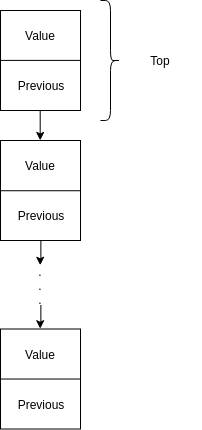
\includegraphics[width=0.25\textwidth]{Images/DataStructures/Stack/Stack.png}
    \caption{Diagram of a Stack}
    \label{fig:stack_diagram-01}
\end{figure}

As you can see our Stack have n elements, where the last element is called top. Also each element of our stack (lets call each element as node) has two things inside, the first one is value and the second is previous where previous is a pointer to the element below of the current node.

To our stack we have two elements, as I mentioned before, we have a pointer called Top, this pointer has the last element of our Stack. The second element is size, it counts the number of elements inside our stack.

If we code the stack with all the operations that I mentioned in the section ''Basic data strcutures'' we have the next as a result:

\begin{lstlisting}
    struct Node{
        Node *previous;
        int value;

        Node(int _value){
            value = _value;
            previous = NULL;
        }
    };

    struct Stack {

        Node *top;
        int size;

        Stack(){
            top = NULL;
            size = 0;
        }

        void Push(int value){
            Node *node = new Node( value );
            if( size == 0 )
                top = node;
            else {
                node -> previous = top;
                top = node;
            }
            size++;
        }

        int Pop(){
            int v_return = INT_MIN;
            if( size > 0){

                v_return = top -> value;
                top = top -> previous;
                size--;

            } else {
                cout << "\nStack is empty \n";
            } 

            return v_return;
        }

        bool IsEmpty(){
            return (size == 0);
        }

        int Top(){
            return top -> value;
        }

        int GetSize(){
            return size;
        }

    };
\end{lstlisting}

In case of competitive programming we can not program a Stack and then use it, beacuse it takes a lot of time, so C++ has a implementation of this data structure in ''stack'' library, and we can use it using the word Stack and defining the data type of our Stack, something like stack $<$ data\_type $>$ or show the example below:

\begin{lstlisting}
    #include <stack>
    using namespace std;

    int main(){
        //Creation of an Stack of int
        stack<int> Stack;
        //Adding an element to our stack
        Stack.push(0);
        //Gets the number of elements of our Stack
        Stack.size();
        //Gets the value of the top element
        Stack.top();
        //The same as top but also removes the top element
        Stack.pop();
        return 0:
    }
\end{lstlisting}

\subsection{Some problems}
\subsubsection{Problem 01}
\textsf{Evalue postfix expression using a stack}
\begin{lstlisting}
    #include <bits/stdc++.h>

    using namespace std;

    int main(){
        string s;
        int number_01 = 0, number_02 = 0;
        stack< int > Stack;
        cin >> s;

        for( auto c : s ){
            if( isdigit(c) ){
                Stack.push( c - '0' );
            } else {

                number_01 = Stack.top();
                Stack.pop();
                number_02 = Stack.top();
                Stack.pop();

                if ( c == '+')
                    Stack.push( number_02 + number_01 );
                else if ( c == '-' )
                    Stack.push( number_02 - number_01 );
                else if ( c == '*' )
                    Stack.push( number_02 * number_01 );
                else if ( c == '/' )
                    Stack.push( number_02 / number_01 );
            }
            
        }
        cout << Stack.top() << endl;
        return 0;
    }
\end{lstlisting}

\subsubsection{Problem 02}
\textsf{Sort values in a stack}
\begin{lstlisting}
    #include <bits/stdc++.h>

    using namespace std;

    stack< int > StackSort(stack<int> &Stack){

        stack<int> AStack;
        
        while( !Stack.empty() ){
            int aux = Stack.top();
            Stack.pop();
            
            while( !AStack.empty() && AStack.top() > aux ){
    
                Stack.push( AStack.top() );
                AStack.pop();    

            }

            AStack.push( aux );
        }
        return AStack;
    }

    int main(){
        stack<int> Stack;
        int n, v;
        cin >> n;
        while(n--){
            cin >> v;
            Stack.push(v); 
        } 

        Stack = StackSort( Stack );

        while( !Stack.empty() ){
            cout << Stack.top() << endl;
            Stack.pop();
        }

        return 0;
    }
\end{lstlisting}

\subsubsection{Problem 03}
\textsf{Check balanced parentheses in an expression}
Solve this problem is not difficult just you need to check which element between our two arrays is smaller than the other, and we will do this until one of our indexes is in the limit. Finally we need to check if one of our arrays was not checked completely. 
\begin{lstlisting}
    #include <bits/stdc++.h>

    using namespace std;

    int main(){

        int m, n;
        vector<int> M, N, ans;

        cin >> m >> n;
        M.resize(m, 0);
        N.resize(n, 0);

        for(int i = 0; i < m; i++)
            cin >> M[i];

        for(int i = 0; i < n; i++)
            cin >> N[i];

        int i = 0, j = 0;
        while( i < m && j < n ){
            if(M[i] < N[j]){
                ans.push_back( M[i++] );
            } else {
                ans.push_back( N[j++] );
            }
        }

        for ( ; i < m; i++)
            ans.push_back( M[i] );

        for( ; j < n; j++)
            ans.push_back( N[j] );

        for( auto e : ans )
            cout << e << " ";
        
        cout << endl;
        return 0;
    }
\end{lstlisting}
